\documentclass[sigconf]{acmart}

% shorten paper
%\usepackage[small,compact]{titlesec}
%
%\usepackage[bf]{caption}
\usepackage{amssymb}
\usepackage{amsmath}
\usepackage{amsfonts}
%\usepackage{amsthm}
% common
%\usepackage{cite} % citex error
\usepackage{url, xspace} 
%\usepackage{graphicx, cite, algorithm, algorithmic, color}
\usepackage{algorithm}
\usepackage{graphicx}
\usepackage{subfig}
\usepackage{bm}
%\usepackage{times} % => compiling error: Package textcomp Error: Symbol \textuparrow not provided by font family ppl in TS1 encoding. Default family used instead
%\usepackage{graphics}
%\usepackage{subfigure}
\usepackage{soul, color}
\soulregister\cite7
\soulregister\ref7
\usepackage{algpseudocode}

%\usepackage{subfigure}

\usepackage{hyperref}
\hypersetup{
  colorlinks=true,      % false: boxed links; true: colored links
  linkcolor=blue,       % color of internal links
  citecolor=magenta,    % color of links to bibliography
  filecolor=cyan,       % color of file links
  urlcolor=red          % color of external links
}

\usepackage{multirow}% http://ctan.org/pkg/multirow
\usepackage{hhline}% http://ctan.org/pkg/hhline

% Paragraph formatting/spacing
%\usepackage[compact]{titlesec}
%\titleformat*{\subsection}{\bf\normalsize}
%\titleformat*{\subsubsection}{\bf\normalsize}
%\titleformat*{\paragraph}{\bf}
% \titlespacing{\section}{0pt}{*1}{*}
% \titlespacing{\subsection}{0pt}{*1}{*}
% \titlespacing{\subsubsection}{0pt}{*1}{*}
% \titlespacing{\paragraph}{0pt}{*1}{*}
\setlength{\parskip}{0pt}

\setlength{\textfloatsep}{  7pt plus 1.0pt minus 2.0pt} % 20.0pt plus 2.0pt minus 4.0pt
\setlength{\floatsep}    {  4pt plus 1.0pt minus 2.0pt} % 12.0pt plus 2.0pt minus 2.0pt
\setlength{\intextsep}   {  4pt plus 1.0pt minus 2.0pt} % 12.0pt plus 2.0pt minus 2.0pt

% \addtolength{\belowcaptionskip}{-2mm}
% \addtolength{\abovecaptionskip}{-1mm}


\usepackage{booktabs} % For formal tables

\newcommand{\reference}[2]{
	\ifthenelse{\boolean{isTechReport}}
	    {\ref{#1}} 
	    {#2}}

\newcommand{\myvec}[1]{\protect\overrightarrow{#1}}


%\newcommand{\desc}[1]{\hl{#1}}
\newcommand{\desc}[1]{}

%\newcommand{\delete}[1]{\st{#1}}
%\newcommand{\new}[1]{\hl{#1}}
\newcommand{\delete}[1]{}
\newcommand{\new}[1]{#1}



\newcommand{\nhattan}[1]{\textcolor{green}{Tan says: #1}}
%\newcommand{\zhenhua}[1]{}

\newcommand{\zhenhua}[1]{\textcolor{red}{Zhenhua says: #1}}
%\newcommand{\zhenhua}[1]{}

\newcommand{\mosharaf}[1]{\textcolor{red}{Mosharaf says: #1}}
%\newcommand{\ramesh}[1]{}

\newcommand{\xiao}[1]{\textcolor{blue}{Xiao says: #1}}

\newcommand{\todo}[1]{\textcolor{red}{(TODO: #1)}}
%\newcommand{\todo}[1]{}

\newcommand{\diff}[1]{\textcolor{red}{#1}}

\newcommand{\argmin}{\arg\!\min}

%\newtheorem{theorem}{Theorem}[section]
%\newtheorem{theorem}{Theorem}
%\newtheorem{corollary}{Corollary}[theorem]
%\newtheorem{lemma}[theorem]{Lemma}
\newtheorem{assumption}{Assumption}

\newcommand{\Exp}[1]{\mathbb{E}\left[#1\right]}
\newcommand{\ra}{\rightarrow}
\newcommand{\R}{\mathbb{R}}

%\newcommand{\Vector}[1]{\textit{\textbf{#1}}}
\newcommand{\Vector}[1]{\boldsymbol{#1}}

\newcommand{\ignore}[1]{}

\newenvironment{compactlist}{
 \begin{list}{{$\bullet$}}{
  \setlength\partopsep{0pt}
  \setlength\parskip{0pt}
  \setlength\parsep{0pt}
  \setlength\topsep{2pt}
  \setlength\itemsep{4pt}
  \setlength{\itemindent}{\leftmargin}
  \setlength{\leftmargin}{0pt}
 }
}{
 \end{list}
}

\newenvironment{denseitemize}{
\begin{itemize}[topsep=2.5pt, partopsep=0pt, leftmargin=1.5em]
  \setlength{\itemsep}{2.5pt}
  \setlength{\parskip}{0pt}
  \setlength{\parsep}{0pt}
}{\end{itemize}}

\newenvironment{denseenum}{
\begin{enumerate}[topsep=2.5pt, partopsep=0pt, leftmargin=1.5em]
  \setlength{\itemsep}{2.5pt}
  \setlength{\parskip}{0pt}
  \setlength{\parsep}{0pt}
}{\end{enumerate}}

\newenvironment{densedesc}{
\begin{description}[topsep=2.5pt, partopsep=0pt, leftmargin=1.5em]
  \setlength{\itemsep}{2.5pt}
  \setlength{\parskip}{0pt}
  \setlength{\parsep}{0pt}
}{\end{description}}

\def\name{BoPF\xspace}

\def\bursty{Bursty}
\def\batch{Batch\xspace}

\def\ala{{\`{a} la}~}
\def\ie{{i.e.}}
\def\eg{{e.g.}}
\def\etal{{et al.}~}
\def\wrt{{w.r.t.}~}
\def\viz{viz.~}
\def\vs{vs.~}
\def\etc{etc.}


\makeatletter
\def\BState{\State\hskip-\ALG@thistlm}
\makeatother


\newcommand{\cL}{{\cal L}}
\def\batchq{TQ\xspace}
\def\burstq{LQ\xspace}


% Copyright
\setcopyright{none}
%\setcopyright{acmcopyright}
%\setcopyright{acmlicensed}
%\setcopyright{rightsretained}
%\setcopyright{usgov}
%\setcopyright{usgovmixed}
%\setcopyright{cagov}
%\setcopyright{cagovmixed}


% DOI
\acmDOI{}

% ISBN
\acmISBN{}

%Conference
\acmConference[SIGMETRICS'18 WIP]{ACM SIGMETRICS}{Irvine}{California, USA} 
\acmYear{2018}
\copyrightyear{2018}

\acmPrice{15.00}

\settopmatter{printacmref=false, printccs=false, printfolios=false}

\begin{document}
\title{\name: Mitigating the Burstiness-Fairness Tradeoff in Multi-Resource Clusters}
%\titlenote{Produces the permission block, and copyright information}
%\subtitle{Extended Abstract}
%\subtitlenote{The full version of the author's guide is available as
%  \texttt{acmart.pdf} document}

%\author{Poster \#3, {\pageref{EndOfPaper} Pages}}
\author{Tan N. Le$^{1,2}$, Xiao Sun$^{1}$, Mosharaf Chowdhury$^{3}$, and Zhenhua Liu$^{1}$}
\affiliation{%
\institution{$^1$Stony Brook University, $^2$SUNY Korea, $^3$ University of Michigan}
}
% \authornote{Submitted papers may not exceed 12 pages in the 2-column ACM format. Figures and tables must be included within the 12 page constraint, but references may extend beyond the 12 pages. Additionally, authors may supplement their paper with an appendix. The length of the appendix is not constrained.}

% The default list of authors is too long for headers}
%\renewcommand{\shortauthors}{B. Trovato et al.}


%
% The code below should be generated by the tool at
% http://dl.acm.org/ccs.cfm
% Please copy and paste the code instead of the example below. 
%
%\begin{CCSXML}
%<ccs2012>
% <concept>
%  <concept_id>10010520.10010553.10010562</concept_id>
%  <concept_desc>Computer systems organization~Embedded systems</concept_desc>
%  <concept_significance>500</concept_significance>
% </concept>
% <concept>
%  <concept_id>10010520.10010575.10010755</concept_id>
%  <concept_desc>Computer systems organization~Redundancy</concept_desc>
%  <concept_significance>300</concept_significance>
% </concept>
% <concept>
%  <concept_id>10010520.10010553.10010554</concept_id>
%  <concept_desc>Computer systems organization~Robotics</concept_desc>
%  <concept_significance>100</concept_significance>
% </concept>
% <concept>
%  <concept_id>10003033.10003083.10003095</concept_id>
%  <concept_desc>Networks~Network reliability</concept_desc>
%  <concept_significance>100</concept_significance>
% </concept>
%</ccs2012>  
%\end{CCSXML}

%\ccsdesc[500]{Computer systems organization~Embedded systems}
%\ccsdesc[300]{Computer systems organization~Redundancy}
%\ccsdesc{Computer systems organization~Robotics}
%\ccsdesc[100]{Networks~Network reliability}


% \keywords{ACM proceedings, \LaTeX, text tagging}



\maketitle

%\input{samplebody-conf.tex}

\section{Background \& Motivation}
\label{sec:background}

\subsection{Interchangeable resources}
\label{sec:speedup}

\desc{GPUs are designed for heavy computing applications}

% GPUs become more important than ever because of the rapid increase in compute-intensive applications.
Modern GPUs are not only graphics processors but can also process massive data in parallel using hundreds or thousands of reduced-instruction-set cores.
Consequently, GPUs have been in wide use for deep-learning applications like image classification, video analytics, speech recognition, and natural language processing \cite{image_classfication_deep,image_classification_cnn,cuda_video_coding, nn_nlp, deep_cnn_nlp}.

% \begin{figure}[h]
% 	\centering
% 	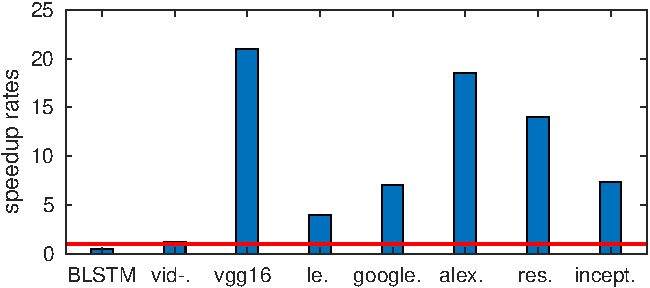
\includegraphics[width=1.0\linewidth]{figs/speedup_rates} \vspace{-0.2in}\caption{Jobs have different speedups from Nvidia K80 GPU versus Intel Xeon E5 2.4 GHz 20-core CPU.}\vspace{-0.1in}
% 	\label{fig:speedup_rates}
% \end{figure}

\desc{GPUs are not always cost effective.}

Different jobs obtain distinct speedups by using GPUs versus CPUs, as shown in Figure~\eqref{fig:speedup_rates}. The speedup rate is how much GPU can reduce the job processing time, i.e., job processing time on a particular CPU divided by that on one GPU. 

While GPUs are generally more efficient for machine learning jobs (with a speedup rate larger than 1), they are more expensive. Figure~\eqref{fig:cost_perf} shows that the normalized costs (the cost ratio between GPUs and CPUs divided by the speedup) vary a lot. When the normalized cost is greater than 1, using GPU is not cost-effective. 

\begin{figure}[h]
	\centering
	%    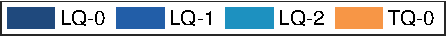
\includegraphics[width=0.6\linewidth]{fig/b1i3_res_usage_legend} 
	\subfloat[Speedups from Nvidia K80 GPU versus Intel Xeon E5 2.4 GHz 20-core CPU.] {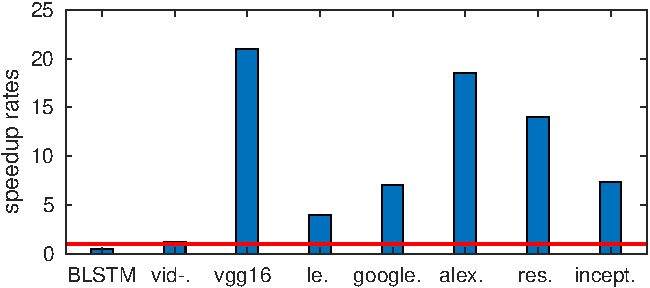
\includegraphics[width=1.0\linewidth]{figs/speedup_rates} \label{fig:speedup_rates}}    \hspace{0.0in}
	\subfloat[Normalized costs using CPUs (c5.large) versus GPU node (p2.xlarge) on EC2] {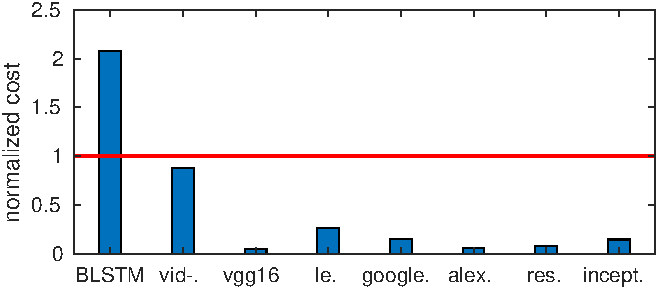
\includegraphics[width=1.0\linewidth]{figs/cost_perf_cloud} \label{fig:cost_perf_cloud}} 
	\caption{GPUs provide distinct speedup and cost-effectiveness.}
	\label{fig:cost_perf}
\end{figure}



%Despite their increasing popularity, GPUs are not always cost effective.
%Figure~\ref{fig:cost_perf} shows normalized costs of CPU and GPU on different benchmarks running on TensorFlow.
% We consider both their off-the-shelf prices and prices on Amazon EC2.
% The normalized cost is the ratio of the GPU price and CPU price, further divided by the speedup rate. The speedup rate is how much GPU can reduce the job processing time, i.e., job processing time on a particular CPU divided by that on one GPU. 
% While GPUs are generally more efficient for machine learning jobs (with a speedup rate larger than 1), they are more expensive. 
% If the normalized cost is more than 1, using GPU is not cost-effective. 

The ineffectiveness of using GPUs in some jobs is due to several reasons.
Although TensorFlow can speedup the performance of CNN models like VGG16, ResNet50, AlexNet, and Inception3 using GPUs \cite{tensorflow-benchmark}, it does not work well with memory networks like Bidirectional LSTM (Bi-LSTM) \cite{deep-learning-cpu-gpu-benchmark}.
RNN models are often updated for each training example for the dependency between two time frames which creates difficulty for parallel computing \cite{huang2013accelerating}.
For the large data input like video-analytics (vid.) \cite{keras-video-classifier}, GPUs are not effective due to the bottleneck in memory and I/O. Therefore, CPUs are preferred for the pre-processing of the video data for the deep learning models.

%\begin{figure}
%	\centering
%	\includegraphics[width=0.7\linewidth]{figs/beta_mov}
%	\caption{Tensorflow jobs have different speedup rates on GPUs (Nvidia K80) vs CPU Xeon E5 2.3Gz 20 cores.}
%	\label{fig:beta_mov}
%\end{figure}




% \desc{CPU applications are still dominant in CPU/GPU clusters}
% We also observe that CPU-only applications are still dominant in most clusters.
% Traditional for-CPU applications have been developed over many years, and it is impractical to convert all these applications for GPUs.
% Furthermore, if the applications are I/O bound, GPUs are not useful.
% For example, database queries are often bound by disk, memory, or network I/O \cite{li2016hippogriffdb}.
% Finally, GPU memory is relatively small; thus it can be a bottleneck for memory-bound applications.
% If the applications do not require much computation, developers will not convert them into GPU applications.
% Although GPU demand is increasing, the load from GPU applications are still small compared to the CPU applications.
%\todo{find the ratio of CPU load vs. GPU load.}

%%% We cannot argue GPUs are not cost effective because speed-up to costs rates are still high as CPU with more CPU cores are also very expensive.
%GPUs may not be cost effective.
%We define the performance-cost ratio as $\frac{\text{speed-up rate}}{(\text{price of GPU}/\text{price of CPU})}$.
%Nvidia shows that Nvidia Tesla K80 can speed-up up to 10x against Intel Xeon E5v3 3.6 Ghz \cite{gpu-k80-speedup}.
%The price of GPU Nvidia Tesla K80 is \$3990 \cite{} while the price of Intel Xeon E5v3 3.6 Ghz is \$363.5 \cite{}.
%
%\begin{figure*}[h]
%    \centering
%    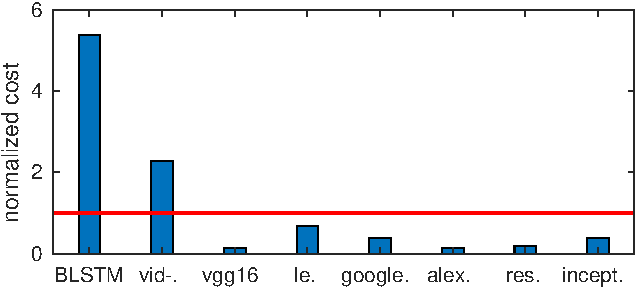
\includegraphics[width=1.0\linewidth]{figs/cost_perf_physical}
%    \caption{Performance-cost ratios show GPUs are not cost-effective because most of ratios are less than 1. Nvidia claims that the speed-up rates of using Nvidia Tesla K80 speeds up 1-10x \cite{gpu-k80-speedup} against Intel Xeon E5v3 3.6 GHz. The price of GPU is \$3990, while the price of CPU is \$363.5.}
%    \label{fig:cost_perf_physical}
%\end{figure*}

\desc{Traditional CPU clusters are low in utilization that gives space for running GPU workloads on CPU.}

In addition to being cost-effective for some jobs, CPUs are often under-utilized.
To this end, we analyzed the Azure Public Dataset \cite{AzurePublicDataset}, which recorded CPU utilization of 5,958 users over 30 days.
We found that more than 90\% users use less than 20\% of their allocated CPU (Figure~\ref{fig:avg_util}).
Because jobs can be executed on CPUs when GPUs are busy, we could utilize the available CPUs before spending a lot in adding more, expensive GPUs.

\begin{figure}[h]
	\centering
	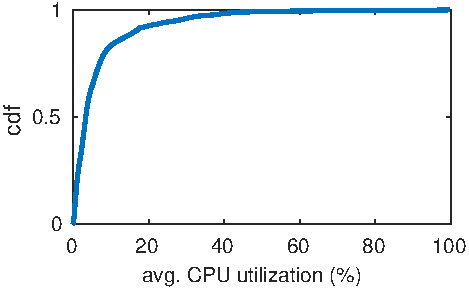
\includegraphics[width=0.8\linewidth]{figs/avg_util}
	\caption{Most of Microsoft Azure users (92.6\% of 5,958 users) have average CPU utilization under 20\%.}
	\label{fig:avg_util}
\end{figure}


\desc{There are interchangeable resources.}

% Thanks to frameworks like TensorFlow \cite{tensorflow}, machine learning applications can run on both CPUs and GPUs.
% Meaning, GPUs can be interchanged with CPUs and vice versa.
% Interchangeable resources like CPUs and GPUs are not rare in large heterogeneous clusters: 
% Heterogeneous CPUs can be interchanged because a more powerful CPU can give better performance than the weaker ones.
% Similarly, one can interchange different network interfaces with different bandwidths, and SSDs with HDDs.

%\subsection{Limitations of current schedulers for CPU/GPU clusters}

\desc{Cannot handle interchangeable resources.}

Unfortunately, existing cluster schedulers do not support interchangeable resources (Table~\ref{tbl:schedulers}) and it is not easy to extend existing schedulers to handle both performance and fairness in the presence of multiple configurations.
Usually, jobs are pre-configured to run on either CPUs or GPUs, therefore systems do not have the flexibility to determine whether to place a job on CPU or GPU. For example, jobs preferring to use GPUs may wait in the GPU queue for a long time, even if CPUs are available and could be a better option in some cases.
Moreover, the configurations are pre-configured by users, who may not know the system-level information to choose the right configurations.


\begin{table}[h]	
	\caption{Resource allocation systems that support GPUs.}
	\label{tbl:schedulers}
	\begin{tabular}{|p{3.5cm}|c|c|}
		\hline
		Systems &  Schedulers & Interchangeability \\ \hline \hline		
		Apache YARN \cite{yarn}    & Fair, DRF & No    \\ \hline
		Kubernetes \cite{kubernetes} & Best effort & No \\ \hline
		Apache Mesos \cite{mesos}   &  DRF          & No  \\ \hline
		Apache Spark \newline (Standalone Mode) \cite{spark}   &  Fair         & No  \\ \hline
	\end{tabular}\vspace{-0.2in}
\end{table}

\desc{Fixed Resource placement is not efficient}

%Since the resource configuration of a job is fixed before its submission, resource interchangeability becomes impossible.


\subsection{Inefficiencies of strawman solutions}
\label{sec:perf-strawman}
%\xiao{new idea: consider the load. When the load is low, actually both MEC and JSQ+ are optimal. But when the load increases, there is a problem. Our approach shirinks to JSQ+ or MEC when the load is low, but when load increases, we have better performance}


\desc{Problem Definition}
To better understand the shortcomings of simplistic heuristics, let us consider a simple setup. 
Assume there are $n$ users sharing a system consisted of interchangeable resources, where each user submits their jobs over time. 
Each job has up to $k$ configurations to run. 
For simplicity of presentation, we restrict our attention to two configurations, i.e., the GPU and the CPU configurations; however, our algorithm and analysis can be readily extended to more configurations, and  different scenarios such as networking interfaces or storage devices. 
A job scheduler for interchangeable resources needs to decide 
(i) the configuration to use for each job and 
(ii) the order of jobs to optimize performance and fairness objectives. 

By default, we do not allow preemption because it is not well supported in many systems such as Kubernetes. 
Even if it is supported, the overhead of migration is often very high. 


%% tan: deletes this example because it does not help.
\del{
Consider a simple example where there are 1 CPU consisted of 32 cores and 1 GPU in the system. 
Each job has two configurations: either the whole CPU or the whole GPU (with a small amount of CPU, e.g., less than a core, to ensure normal execution). 
There are two users. 
User 1 has 5 jobs, each takes 10 minutes to finish on CPU, and 5 minutes on GPU. User 2 has 5 jobs requires 40 and 10 minutes on CPU and GPU, respectively. 
If we want to minimize the average job completion time (JCT), the optimal solution is to put all jobs of user 1 on CPU and all jobs of user 2 on GPU, resulting in an average JCT of 30 minutes. 
}


%processing time on CPU, or 5 mins on GPU, while Job 2 requires either 40 mins processing time on CPU or 10 mins on GPU. If we try to minimize the average completion time, then clearly we should use GPU for job 2 and CPU for job 1.





%Each version will use corresponding GPU or CPU as the computational resource, and each job can only pick one configuration. Assume every job has the same configuration settings, but the processing time on different resources are different, and we assume the processing time is known. The goal is to decide the configuration for each job and then schedule the jobs to reach a better performance and fairness output.

While (ii) has been studied extensively in existing work~\cite{drf,drfq,carbyne,tetris,hug}, (i) is the new challenge. 
In this section, we revisit existing algorithms for this new problem to illustrate their inefficiencies and demonstrate why we need new algorithms. 
In addition, we show that strawman solutions may lead to poor performance, highlighting that designing a new algorithm is challenging.






%In the following subsection, we will consider performance (in terms of job completion time) and fairness seperately. We will see that a strawman solution fails to solve this problem -  and in most of the time, far from optimal solution.

%\subsubsection{Performance}

We focus on performance in this section, in particular, minimizing the average job completion time (JCT). Fairness is discussed in Section~\ref{sec:fairness}.  

\desc{Each job use its most effective resource}

%For the problem described above, if our goal is to minimize average completion time, the problem is in P if we assume all jobs arrives at time 0. if they arrive over time, then the problem becomes strongly NP-Hard, even if we allow preemption. Before we discuss our polynomial algorithm in section xxx, we start with heuristics and show why they did not work.


The first approach we consider is Most Effective Configurations (MEC): the scheduler asks users to pick one configuration for each job and the scheduler is only responsible for the job ordering and placement. 
Under this approach, the load on CPU and GPU can be largely unbalanced. For instance, if all jobs favor GPUs, no users would pick the CPU configuration, resulting in arbitrarily low utilization of CPU, and vice versa. 
Actually, if there are $k$ interchangeable resources, this approach may result in $k-1$ of them unused. 

The under-utilization of resources has profound impacts on job completion time, especially when the system load is high. For instance, assume all the GPUs together can finish 10 jobs/minutes on average and all the CPUs can finish 10 jobs/minutes possibly with longer processing time for each job. Then if the arrival rate is 15 jobs/minutes, the waiting time when we only use GPUs would keep increasing. Under the ``heavy traffic'' situations, low utilization results in arbitrarily large job completion time. 
%\del{, and these situations are exactly when we greatly need thoughtful scheduling algorithms}.
Therefore, \emph{picking the most effective configuration for each job may result in low utilization and high waiting time}.

%This approach is not optimal, as the load of CPU and GPU can be largely unbalanced, especially for machine learning jobs. For example, if for all jobs, the processing time on GPU is always shorter than CPU, then of course people would choose using GPUs in a shared cluster. While GPU is fully utilized, CPUs are barely used. So the performance can be as bad as the computational power between total GPUs and total CPU cores. For example, if they have the same computational power, then the degeneration can be as much as 50\%.

\desc{users see the load}

The inefficiency of MEC is because the configuration selection does not take into consideration the current system load. Therefore, the second approach is a modified Join the Shortest Queue (JSQ+). 
Assume users know the current waiting time on each resource in real time. On the arrival of a job, the scheduler picks the resource that has the shortest completion time, i.e, the sum of waiting time and the processing time of the job on the corresponding resource. 
In this way, loads on different resources can be more balanced because as the load on some resources increases, their longer waiting time would encourage new jobs to be placed on other resources. 
Note that it is different than the vanilla joining the shortest queue. 
For instance, if a job has the processing times of 10 minutes and 40 minutes on GPU and CPU, respectively, and the waiting times on GPU and CPU are 40 and 20 minutes, respectively.
Although CPU has a shorter waiting time, this job pick GPU because it is much more efficient on GPU, resulting in a completion time of 50 minutes.
If the job was placed on CPU, the completion time would increase to 60 minutes.

%reports back the current node on different resource - so the user can choose whichever node that has the shortest expected finishing time if the job will be running on that node. 

\emph{The key drawback of JSQ+ is that it is short-sighted}: each job attempts to minimize its own completion time without considering the impacts on later jobs. 
Here is an example with 2 CPUs and 2 GPUs. Assume there are 4 jobs, all arrive at the beginning but in the order of Job 1, 2, 3, 4. The processing time can be show in a matrix: 
$$
P = \begin{bmatrix}
40 & 50 \\
40 & 50 \\
40 & 80\\
40 & 80\\
\end{bmatrix}
$$
In this matrix, the $i$-th row consists of job $i$'s processing times on GPUs and CPUs, respectively. For instance, the first row means Job 1 needs 40 minutes on GPU or 50 minutes on CPU.

Under JSQ+, Job 1 first picks a GPU, and then Job 2 picks the other GPU.
After that, Job 3 and Job 4 have no choices but to pick CPUs, as shown in Figure~\eqref{fig:JSQ_ex} with an AJCT of 60 minutes.
%\xiao{This may not be true, as Job 3 and 4 can choose to join the GPU queue and wait instead of using CPU directly}
Clearly, the optimal solution is to put Job 3 and 4 on GPUs and Jobs 1 and 2 on CPUs, which can reduce the AJCT from 60 minutes to 45 minutes as Figure \eqref{fig:JSQ_ex_opt}.

\begin{figure}[h]
	\centering
%	{
\includegraphics[width=0.7\linewidth]{figs/JSQ_ex_legend} \label{fig:JSQ_ex_legend}}    \hspace{0.0in}
	\subfloat[JSQ+] {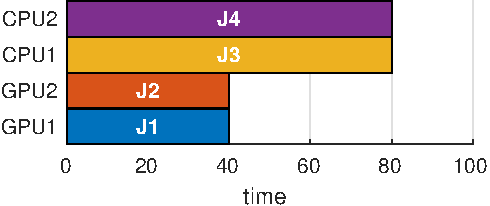
\includegraphics[width=0.7\linewidth]{figs/JSQ_ex} \label{fig:JSQ_ex}}    \hspace{0.0in}
	\subfloat[Optimal] {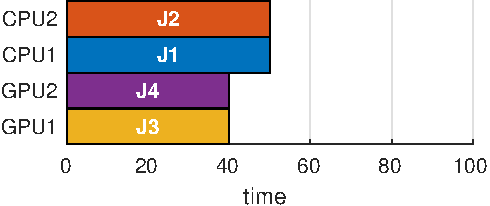
\includegraphics[width=0.7\linewidth]{figs/JSQ_ex_opt} \label{fig:JSQ_ex_opt}}    \hspace{0.0in}	
	\caption{Under JSQ+, Job 1 and 2 are scheduled on GPU, while Job 3 and 4 are scheduled on CPU. In contrast, \name runs Job 3 and Job 4 on GPUs because they have higher speedup on GPUs. } %\tanle{We don't need 4 jobs in the motivation examples. Should I make it to two jobs or vary the lengths a bit?}}
	\label{fig:JSQ}
\end{figure}

%Clearly, this is not an optimal solution, as there is more gain by scheduling Job 3 and 4 to GPUs.


\desc{System pick configuration}

The sub-optimality of these two strawman solutions implies that we cannot just let each user pick her own job configurations, even if users are equipped with the current system load information. 
Therefore, the scheduler needs to coordinate the decisions, where Shortest Job First (SJF) is widely used.
%So now we consider a centralized approach by comparing all configurations between jobs. 

When there are multiple configurations for each job, we can extend SJF to SJF+ to handle jobs with multiple configurations: for each type of resource, maintain a queue of all available jobs. The jobs are sorted based on the processing time on this resource, e.g., GPU, in an increasing order. Whenever a resource becomes available, schedule the first job in the corresponding queue to this resource and remove the job from all queues. When multiple resources are available at the same time, first schedule a job to the one with shorter processing time. 

This algorithm is optimal when there is only 1 configuration~\cite{cobham1954priority}. 
%\todo{Xiao, can you add the citation?}
When there are more than 2 configurations, however, the performance can be \emph{arbitrarily bad}. Consider the following example:

$$
P = \begin{bmatrix}
10 & 20\\
10 & 20 \\
20 & 90\\
20 & 90\\
\end{bmatrix}
$$


\begin{figure}[h]
	\centering
%	
\includegraphics[width=0.7\linewidth]{figs/SJFplus_ex_legend} \hspace{0.0in}
	\subfloat[SJF+] {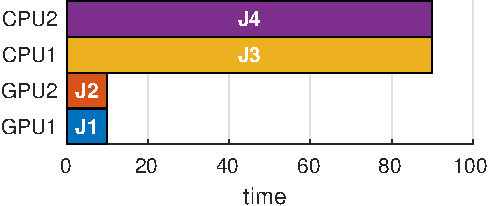
\includegraphics[width=0.7\linewidth]{figs/SJFplus_ex} \label{fig:SJFplus_ex}}    \hspace{0.0in}
	\subfloat[Optimal] {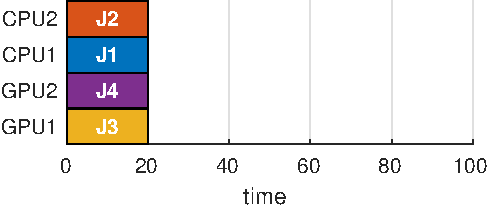
\includegraphics[width=0.7\linewidth]{figs/SJFplus_ex_opt} \label{fig:SJFplus_ex_opt}}    \hspace{0.0in}
%	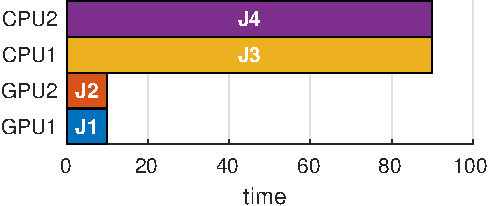
\includegraphics[width=0.8\linewidth]{figs/SJFplus_ex}
	\caption{Under SJF+, Job 1 and 2 are scheduled on GPU, while Job 3 and 4 are placed on CPU. In contrast, \name places Job 3 and Job 4 on GPUs because the time reductions on GPUs of these two jobs are larger.}
	\label{fig:SJF}
\end{figure}


Under SJF+, there are two queues for GPU and CPU, respectively. The order in both queues is Job 1, Job 2, Job 3, Job 4. Therefore, Job 1 and 2 are placed on GPUs first. Then Job 3 and 4 are scheduled on CPUs. This is shown in Figure~\ref{fig:SJF}, resulting in an AJCT of 50 minutes. 
%Job 3 and 4 are large jobs and they have more gains by putting them into GPUs, however, because of the non-idle property of SJF scheduling, Job 3 and 4 are forced to be scheduled on an inefficient resource.
In contrast, the optimal solution places Jobs 3 and 4 on GPUs and Jobs 1 and 2 on CPUs, reducing the AJCT to 20 minutes. 
The root cause is while Jobs 3 and 4 are longer (disadvantage in SJF+), the processing time reduction of using GPU is much larger (overlooked by SJF+).


To summarize, when jobs have multiple configurations, even if jobs arrive at the same time, the problem is more challenging than that with single configuration because we need to consider the processing time reduction among different configurations, which may contradict with other factors, e.g., the length of the job. Therefore, algorithms that perform well for single configuration job scheduling may result in arbitrarily bad performance in the new problem.  

%with 2 configurations for each job, all existing heuristics failed to provide a good guarantee, even for the simplest case. The root is that, it seems to have more gains, we should schedule large jobs on efficient resource, but from traditional scheduling perspective, to minimize average completion time, we should start with smaller jobs. 


In \S\ref{sec:alg}, we will provide a network algorithm, and show its optimality for average job completion time.





% \subsection{Illustrations of \name}

% \desc{Strawman solutions do not work.}

% To handle interchangeability, a strawman solution would equally shares the resources among users and then places the jobs into resource in the best-effort manner.
% To illustrate the inefficiency of the strawman solution and the potential of \name, we create an simple example in Table \ref{tbl:mov_example}.
% There are 2 users, i.e., User 1 and User 2.
% Each user has 3 jobs.
% Each job can execute either on CPU or GPU with different completion times.
% The GPU/CPU speed-up rates of jobs are different.
% 6 jobs are queued up at the beginning.

% \begin{table}[H]    
% 	\caption{Motivation example.}
% 	\label{tbl:mov_example}
% 	\begin{tabular}{|c|c|c|c|}
% 		\hline
% 		User & Job ID & Compl. on GPU & Compl. on CPU \\  \hline \hline
% 		User 1 & 1 & 3 & 4 \\  \hline
% 		User 2 & 2 & 3 & 3 \\  \hline
% 		User 1 & 3 & 1.5 & 4 \\  \hline
% 		User 2 & 4 & 2 & 3 \\  \hline
% 		User 1 & 5 & 1 & 2 \\  \hline
% 		User 2 & 6 & 1.5 & 2 \\  \hline
% 	\end{tabular}
% \end{table}

% Figure \ref{fig:motivation_example} compares the strawman solution and \name.
% The strawman solution in Figure \ref{fig:motivation_example_1} equally shares CPU and GPU for two users and places the jobs in CPUs and GPUs.
% The average completion time of 6 jobs in Figure \ref{fig:motivation_example_1} is $\frac{20}{6}$.
% The strawman solution fully utilizes the resources but its performance is far from optimal.
% Figure \ref{fig:motivation_example_2} illustrates our solution that is clearly better than the strawman one.
% The average completion in Figure \ref{fig:motivation_example_2} is $\frac{13}{6}$ that achieves $35\%$ performance improvement.

% \begin{figure}[H]
% 	\centering
% 	% 3+4+3+5+2+3
% 	\subfloat[Fair share \& Best effort] {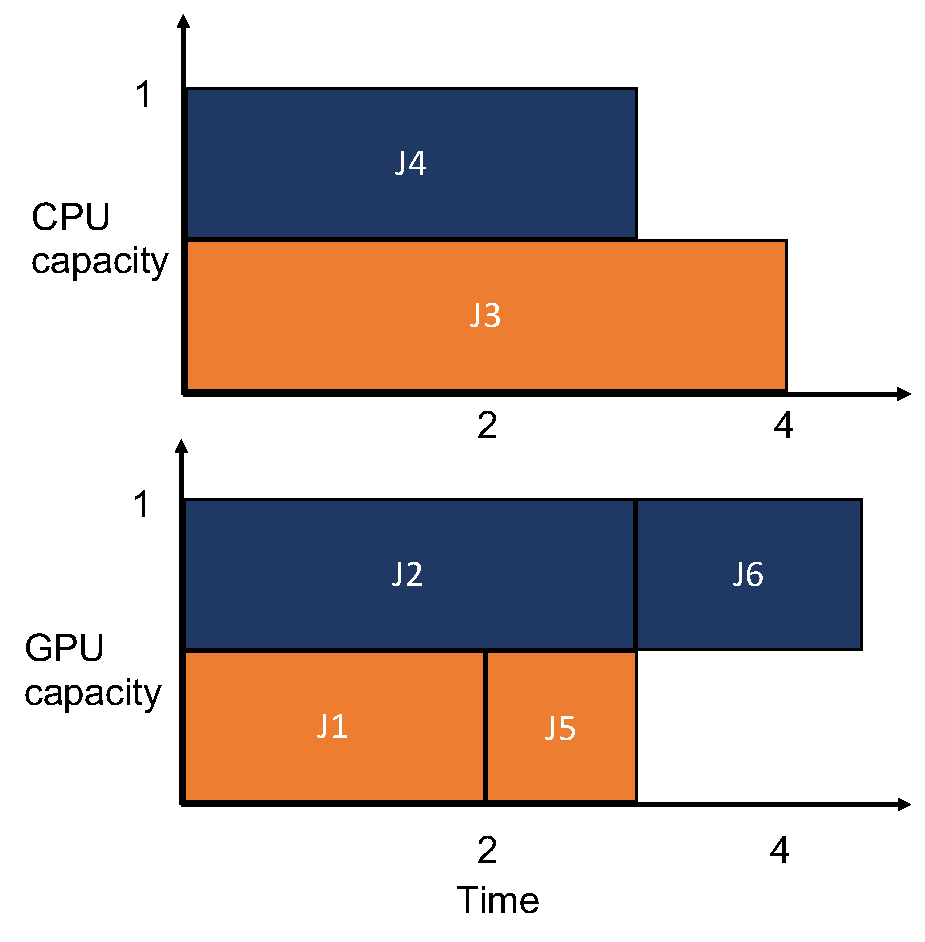
\includegraphics[width=0.45\linewidth]{figs/motivation_example_1} \label{fig:motivation_example_1}} 
% 	% 3+2+1.5+3+1+2.5
% 	\subfloat[\name allocation \& scheduling ]{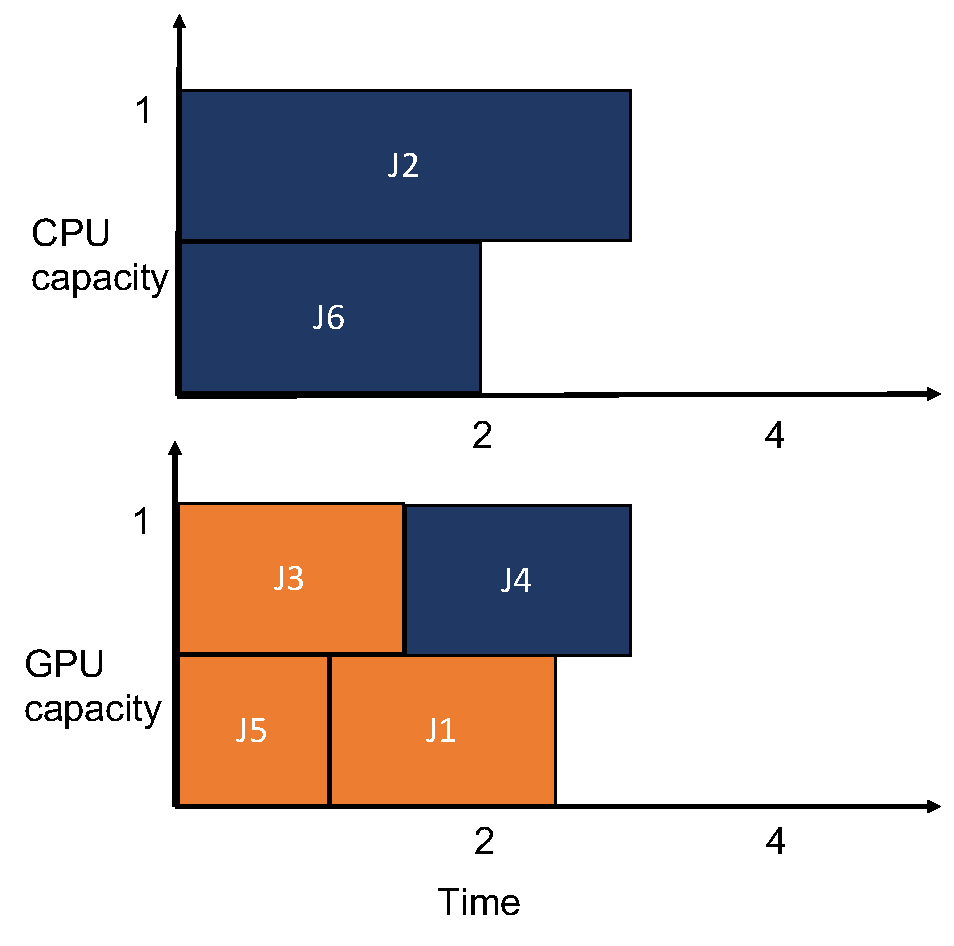
\includegraphics[width=0.45\linewidth]{figs/motivation_example_2} \label{fig:motivation_example_2}}
% 	\caption{Opportunities for job scheduling in CPU/GPU clusters.
% 	Figure \ref{fig:motivation_example_1} depicts the allocation of the strawman solution using fair-share and best-effort scheduling in the FIFO maner.
% 	Although the strawman solution fully utilizes resources, it does not give the optimal solution.
% 	Meanwhile, \name exploits the interchangeability between CPUs and GPUs to improve 35\% performance.}
% 	\label{fig:motivation_example}
% \end{figure}

% \xiao{Motivation starts here} \\
% As our goal is manifold: fairness, efficiency and performance, we show that current existing schedulers and algorithms fail to provide satisfiable result in at least 1 or more aspect.



%This approach works well in the offline case where we can perfect measure the $\beta$. If the $\beta$ is properly choose, we can prove that this algorithm is Pareto-efficient, Envy-free and sharing-incentive. 

%However, under online case, we can not get perfect $\beta$, and the estimation will be changing overtime, so the dominant share of all users are fluctuating, thus those properties can hardly hold in online case.

% \subsubsection{Efficiency}

% In traditional multi-resource allocation problem, the efficiency, or the system utilization is often optimized based on some greedy 'packing' heuristics. As long as the resource is not wasted at every time slot, we should observe a better makespan, so that the efficiency will be improved.  However, under \name, this is no longer true due to job placement onto an improper computation resource. Consider the following example:

% Assume the cluster size is (24 CPU cores, 2 GPUs and 48 GB memory) there is only 1 user in the system and the user has 2 different categories of jobs. 9 jobs are from Type A, which require 8 CPU cores and 8 GB memory, with 10 units processing time and 1 GPU and 2 GB memory with 3 units processing time. 2 jobs are from Type B, which require 16 CPU cores and 16 GB memory, with 8 units processing time on CPU and 1 GPU and 2 GB memory with 30 units processing time.

% The comparison of a packing scheduler and a non-packing scheduler is shown at figure \ref{fig:efficiency}.
% \begin{figure}
% 	\centering
% 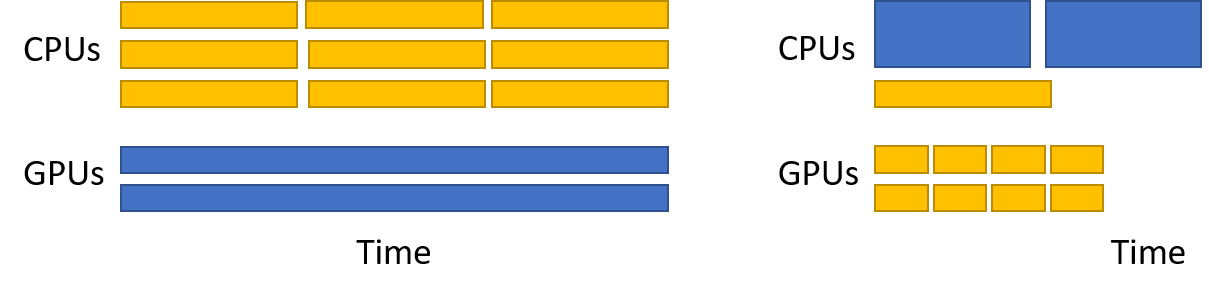
\includegraphics[width=0.8\linewidth]{figs/efficiency}
% 	\caption{Perfect packing does not leads to good utilization. The makespan for left figure is 30, and it is 16 for right figure with imperfect packing.}
% 	\label{fig:efficiency}
% \end{figure}


% \subsubsection{Performance}
% The performance evaluated for a user is based on the average completion time of all jobs from that user. Usually for this objective function,  the widely applied heuristic policy is shortest  job first - simply sort all jobs and schedule the job with shortest processing time. We show that simple vanilla greedy SPT algorithm would also face challenges under our interchangeable settings.

% Similar to previous setting, assume we have a cluster of size (24 CPU cores, 2 GPUs and 48 GB memory) and there is only 1 user in the system, so we don't have to consider fairness. There are 2 types of jobs, all of them have identical job demand but have different processing time. For type A jobs, they require 8 time units on both CPU and GPU. For type B jobs, they require 10 units on GPU and 20 units on CPU. The schedule for SPT and optimal is shown at Figure \ref{fig:performance}.

% \begin{figure}
% 	\centering
% 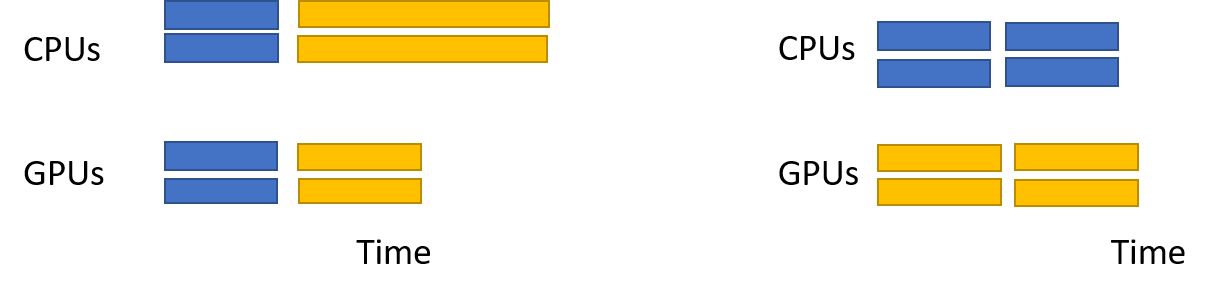
\includegraphics[width=0.8\linewidth]{figs/performance}
% 	\caption{SPT is not necessarily optimal. The ACT for SPT is 15.5 while the act for optimal is  13.5.}
% 	\label{fig:performance}
% \end{figure}

% \subsection{Modeling}

% We model our \name allocation and scheduling problem starting from the workload. In a typical hybrid cluster, assume $C_1,C_2,C_3$ represents the capacity of CPU cores, GPUs and memory from the cluster. there are $n$ active users, and each of them keep submitting machine learning jobs. For each job $j$, when it arrives at time $r_j$, it contains 2 configurations representing the resources demand  
% $$
% 	Q_i=
% 	\begin{bmatrix}
% 	c_i & m_i^1 & p_i^1 \\
% 	g_i & m_i^2 & p_i^2 
% 	\end{bmatrix} $$
% where the first row shows the demand and estimated processing time if the job  will be placed in CPU and the second row show the corresponding GPU configurations.

% Consider the  non-preemptive offline scheduling problem first, the constraints can be formulated as the following:

% \begin{equation}
% \begin{array}{ll@{}ll}
% ~ & \displaystyle\sum\limits_{i,s} x_{i,j,s} =1  & \forall j \\
% ~ &  \displaystyle\sum\limits_{j,s\in (t-p_j^i,t]} x_{i,j,s}c_j \leq   C_1  & ~~\forall i,t \\
% ~ &  \displaystyle\sum\limits_{j,s\in (t-p_j^i,t]} x_{i,j,s}g_j \leq   C_2  & ~~\forall i,t \\
% ~ &  \displaystyle\sum\limits_{j,s\in (t-p_j^i,t]} x_{i,j,s}m_j^i \leq   C_3  & ~~\forall i,t \\
% ~& x_{i,j,s} = 0   & ~~\forall i,j,s > T-p_j^i ~or~s<r_j\\
% & x_{i,j,s} = \{0,1\} & \forall i,j,s\\
% \end{array}
% \end{equation}

% with extra trivial nonnegative constraints. In the above integer programming, $T$ is a trivial upper bound on the makespan of any reasonable schedule. $x_{i,j,s}$ indicates whether job $j$ is processed with computation resource $i$ at starting time $s$. 

% The objective function, depending on ACT or makespan, can be formulated as $\sum\limits_{i,s}x_{i,j,s}(s+p_{j}^i)$ or $\max x_{i,j,s}(s+p_{j}^i)$. However, regardless of what objective we choose, the optimization will be a NP-Hard problem. The hardness come from 2 parts: the multi-dimensional queueing problem, and the rigid job scheduling problem. Hence, for current paper, Our goal is to seek heuristic that works well in the real system.





\subsection{Other challenges}



\desc{Simultaneously improve performance, efficiency, and fairness.}

The tradeoff between performance and fairness is well-known \cite{fairness_efficency_tradeoffs,hug}.
For our problem, if we only optimize for performance using ideas such as shortest job first, users with larger jobs may starve so it is not fair at all.
On the other hand, if we aim at instantaneous fairness such as DRF, there is not much room to improve the performance.
Therefore, the key challenge is how to achieve better job completion time with fairness. 

\desc{Need to estimate the performance of job on CPU or GPU}

On the system side, we need to estimate the job completion times in an online manner with reasonable overhead.
This provides inputs for the scheduler in \name and can free users from setting up the configurations. 


% To achieve the improvement in Figure \ref{fig:motivation_example_2}, we  need to have the estimate of completion times of jobs.
% However, performance prediction is challenging \cite{ernest, cherrypick}.
% First, low accuracy may result in largely negative impact on \name.
% Second, prediction may require large overheads which can make the improvement may not be useful.
% In spite of these challenges, we still want to provide this performance prediction with low overheads and high accuracy.

% It is difficult to optimize performance, efficiency, and fairness simultaneouly.
% If we enforce fair resource allocation among users like Figure \ref{fig:motivation_example_1}, it hurts the performance and efficiency.

% To improve performance, the straight-forward solution is to put the jobs with low speed-up rates on CPUs and jobs with high speed-up rates on GPUs.
% However, it is not true that it also maximizes the efficiency and fairness.
% To demonstrate this, we re-use the motivation example in Table \ref{tbl:mov_example}.
% For instance, we place jobs with large speed-up rates $(\geq 1)$ in GPUs, while putting the small speed-up rates $(<1)$ on CPUs.
% In this case, we actually place all 6 jobs on GPUs but do not use any CPUs that results in low efficiency.

% If we try to optimize the performance and efficiency, it is not trivial to maintain fairness among users.
% When resources are interchangeable, it is actually hard to define fairness.
% Traditional schedulers \cite{yarn, mesos} maintain fairness based on the received resources among users.
% However, this definition of fairness cannot be used when resources are not equally important.
% Naive fair allocation may result in inefficiency like Figure \ref{fig:motivation_example_1}.
\section{Design Details}
\label{sec:impl}

In this section, we describe how we have implemented \name on Apache YARN, how we use standard techniques for demand estimation, and additional details related to our implementation.

\begin{figure}
\centering
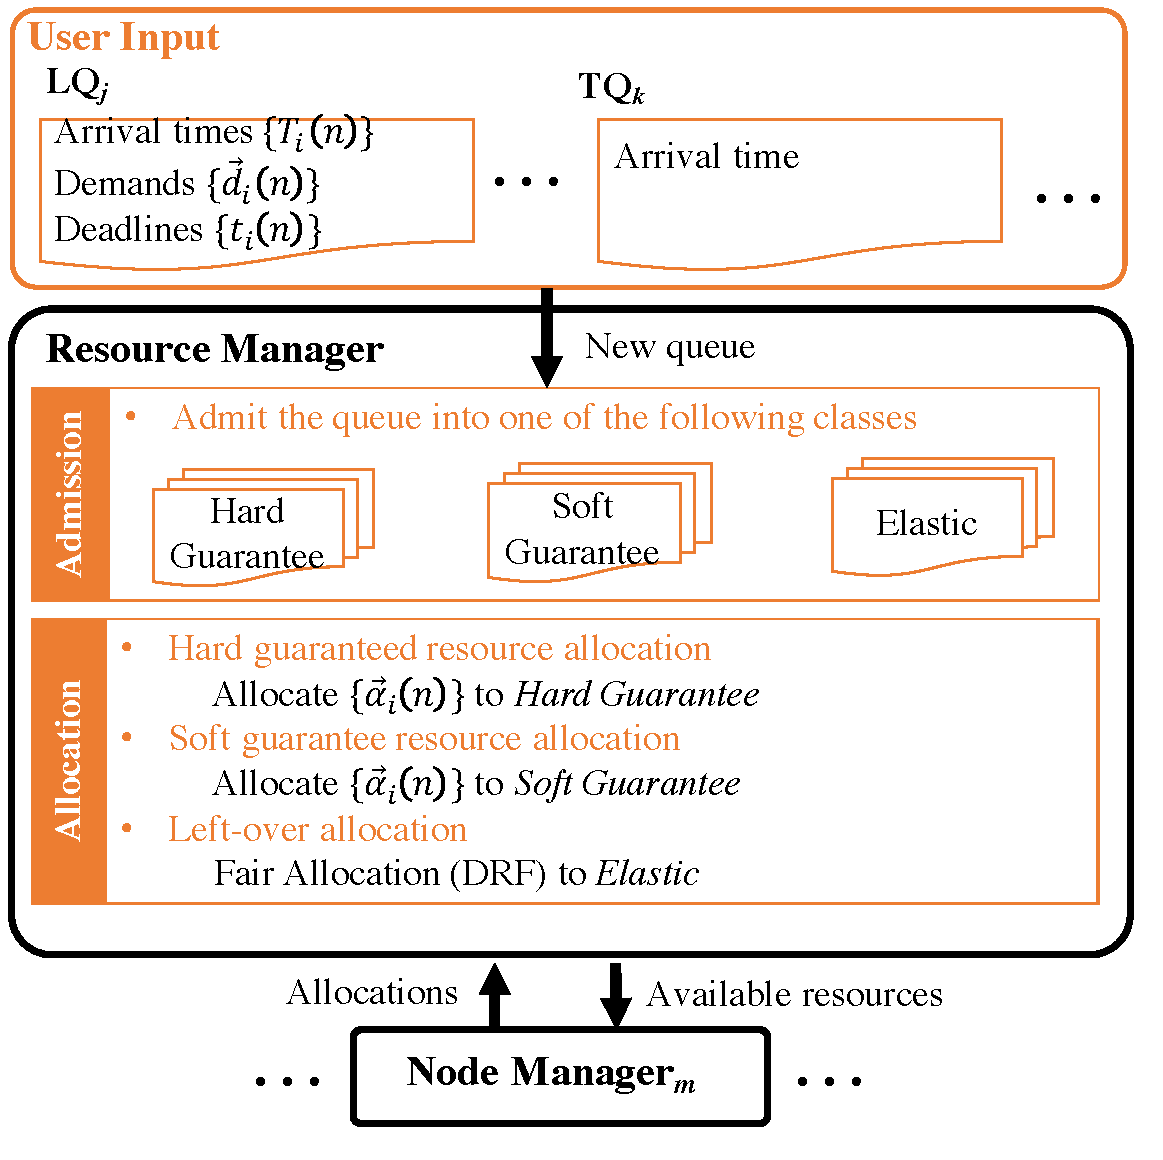
\includegraphics[width=1.0\linewidth]{fig/diagram}
\caption{Enabling bounded prioritization with long-term fairness in a  multi-resource cluster. 
\name-related changes are shown in orange. \todo{change the figure ON durations to deadlines}}
\label{fig:system_design}
\end{figure}

\subsection{Enabling \name in Cluster Managers}
Enabling bounded prioritization with long-term fairness requires implementing the \emph{\name scheduler} itself along with an additional \emph{admission control} module in cluster managers, and it takes \emph{additional information on demand characteristics} from the users. 
A key benefit of {\name} is its simplicity of implementation: we have implemented it in YARN using only $600$ lines of code.
In the following, we describe how and where we have made the necessary changes.

\subsubsection*{Primer on Data-Parallel Cluster Scheduling}
Modern cluster managers typically includes three components: \emph{job manager} or application master (AM), \emph{node manager} (NM), and \emph{resource manager} (RM).

One NM runs on each server in the cluster, and it is responsible for managing resource containers on that server. 
A container is a unit of allocation and are used to run specific tasks. 

For each application, a job manager or AM interacts with the RM to request job demands and receive allocation and progress updates. 
It can run on any server in the cluster. 
AM manages and monitors job demands (memory and CPU) and job status (\texttt{PENDING}, \texttt{IN\_PROGRESS}, or \texttt{FINISHED}). 

The RM is the most important part in terms of scheduling. 
It receives requests from AMs and then schedules resources using an operator-selected scheduling policy. 
It asks NM to prepare resource containers for the various tasks of the submitted jobs.

\subsubsection*{\name Implementation}
We made three changes for taking user input, performing admission control, and calculating resource shares -- all in the RM.
We do not modify NM and AM.
Our implementation also requires more input parameters from the users regarding the demand characteristics of their job queues. 
Figure~\ref{fig:system_design} depicts our design.

\paragraph{User Input} Users submit their jobs to their queues. 
In our system, there are 2 queue types, i.e., {\burstq}s and {\batchq}s. 
We do not need additional parameters for {\batchq}s because they are the same as the conventional queues. 
Hence, we assume that {\batchq}s are already available in the system. 
However, the \name scheduler needs additional parameters for LQs; namely, arrival times and demands.

Users submit a request job that contains their parameters of the new \burstq. 
After receiving the parameters in the job, the RM sets up a new \burstq queue for the user.
Users can also ask the cluster administrator to set up the parameters. 

\paragraph{Admission Control} YARN does not support admission control. 
We implement an admission control module to classify {\burstq}s and {\batchq}s into Hard Guarantee, Soft Guarantee, and Elastic classes. 
A new queue is rejected if it cannot meet the safety condition \eqref{eqn:ad-safety}, which invalids the committed performance.
If it is a \batchq, it is added into the Elastic class.
If the new {\burstq} does not satisfy the fairness condition \eqref{eqn:ad-fair}, it is also admitted to the Elastic class.
If the new {\burstq} meets the fairness condition \eqref{eqn:ad-fair}, but fails at the resource condition \eqref{eqn:ad-enough}, it will be put in the Soft Guarantee class.
If the new {\burstq} meets all the three conditions, i.e., safety, fairness, and resource, it will be admitted to the Hard Guarantee class.

\paragraph{\name Scheduler} We implement \name as a new scheduling policy to achieve our joint goals of bounded priority with long-term fairness. 
Upon registering the queues, users submit their jobs to their {\burstq}s or {\batchq}s. 
Thanks to admission control, {\burstq}s and {\batchq}s are classified into Hard Guarantee, Soft Guarantee, and Elastic classes. 
Note that resource sharing policies are implemented across queues in YARN, jobs in the same queue are scheduled in FIFO manner.
Hence, \name only sets the share at the individual queue level.

\name Scheduler periodically set the share levels to all {\burstq}s in Hard Guarantee and Soft Guarantee classes.
These share levels are actually upper-bounds on resource allocation that an {\burstq} can receive from the cluster. 
Based on the real demand of each {\burstq}, \name allocates resources until it meets the share levels\delete{ (whether it is in the ON period or OFF period)}. 

\name Scheduler allocates the resource to the three classes in the following priority order: (1) Hard Guarantee class, (2) Soft Guarantee class, and (3) Elastic class. 
The {\burstq}s in the Hard Guarantee class are allocated first.
Then, the \name continues allocates the resource to the {\burstq}s in Soft Guarantee class.
The queues in the Elastic class are allocated with left-over resources using DRF \cite{drf}.

%To ensure work conservation, unused resources by all queues are combined and redistributed across queues in the Elastic class using DRF \cite{drf}. 

\subsection{Demand Estimation}

\name requires accurate estimates of resource demands and their durations of \burstq jobs by users. 
These estimations can be done by using well-known techniques; \eg, users can use history of prior runs \cite{rope, jockey, tetris} with the assumption that resource requirements for the tasks in the same stage are similar \cite{drf, pacman, paratimer}. 
We do not make any new contributions on demand estimation in this paper. 
%While {\name} performs the best with accurate estimations, we have found that {\name} is robust to small misestimations in practice (\S\ref{sec:performance_large_scale}).
When LQs have bursty arrivals of different sizes, BPF with the $\alpha$-strategy ensures the performance with the average usage remains similar (\S\ref{sec:performance_large_scale}). 
We consider a more thorough study an important future work. 

\subsection{Operational Issues}

\paragraph{Container Reuse}
Container reuse is a well-known technique that is used in some application frameworks, such as Apache Tez. 
The objective of container reuse is to reduce the overheads of allocating and releasing containers. 
The downside is that it causes resource waste if the container to be reused is larger than the real demand of the new task. 
Furthermore, container reuse is not possible if the new task requires more resource than existing containers. 
For our implementation and deployment, we do not enable container reuse because {\name} periodically prefers more free resources for \burstq jobs, causing its drawbacks to outweigh its benefits in many cases.

\paragraph{Preemption}
Preemption is a recently introduced setting in the YARN Fair Scheduler \cite{hadoop-fair-scheduler}, and it is used to kill running containers of one job to create free containers for another. 
By default, preemption is not enabled in YARN. 
For {\name}, using preemption can help in providing guarantees for {\burstq}s. 
However, killing the tasks of running jobs often results in failures and significant delays. 
We do not use preemption in our system throughout this paper.

%\subsection{Possible issues}

%In the same worker node, containers are sequentially launched. Slow allocation of containers may hurt resource guarantee.

% % old text % %
%\begin{algorithm}
%\caption{Scheduler}
%\label{algorithm1}
%\begin{algorithmic}[1]
%\Procedure{periodicSchedule()}{}
%\State $\{\mathbb{A}, \mathbb{B}, \mathbb{U}\}$ = \textsc{updateQueueStatus}($\mathbb{A}$,$\mathbb{B}$,$\mathbb{U}$)
%\If{\textsc{isNewArrival}($\mathbb{Q}$)}
%	\State Update the best effort queues: $\mathbb{U} = \mathbb{U} \cup \mathbb{Q}$
%\EndIf
%\State $\{\mathbb{A}, \mathbb{B}, \mathbb{U}\}$ = \textsc{admit}($\mathbb{U}$)
%\State \textsc{allocate}($\mathbb{A}$,$\mathbb{B}$)
%\State Obtain the available cluster resources $\myvec{L}$
%\State DRF($\mathbb{U}$, $\myvec{L}$)
%\EndProcedure
%\\
%\Function{updateQueueStatus($\mathbb{A}$,$\mathbb{B}$,$\mathbb{U}$)}{}
%\ForAll{queue $A \in \mathbb{A}$}
%	\If{queue $A$ is deactivated}  Update $\mathbb{A} = \mathbb{A} \setminus A$
%	\EndIf
%\EndFor
%\ForAll{queue $B \in \mathbb{B}$}
%	\If{queue $B$ is deactivated} Update $\mathbb{B} = \mathbb{B} \setminus B$
%	\EndIf	
%\EndFor
%\ForAll{queue $U \in \mathbb{U}$}
%	\If{queue $U$ is deactivated} Update $\mathbb{U} = \mathbb{U} \setminus U$
%	\EndIf
%\EndFor
%\State \textbf{return} $\{\mathbb{A} , \mathbb{B},\mathbb{U}  \}$	
%\EndFunction
%\\
%\Function{admit(queues $\mathbb{U}$)}{}
%\ForAll{queue $U \in \mathbb{U}$}
%	\If{queue $U$ is a bursty queue}
%		\If{admission conditions \eqref{eqn:bursty_adm_cond_2} satisfied}
%			\State Update $\mathbb{A} = \mathbb{A} \cup U$
%			\State Update $\mathbb{U} = \mathbb{U} \setminus U$
%		\EndIf
%	\Else
%		\If{admission condition \eqref{eqn:batch_adm_cond} satisfied}
%			\State Update $\mathbb{B} = \mathbb{B} \cup U$
%			\State Update $\mathbb{U} = \mathbb{U} \setminus U$
%		\EndIf
%	\EndIf
%\EndFor
%\State \textbf{return} $\{\mathbb{A} , \mathbb{B},\mathbb{U}  \}$	
%\EndFunction
%\\
%\Function{\diff{allocate}($\mathbb{A}$, $\mathbb{B}$)}{}
%\ForAll{bursty queue $A \in \mathbb{A}$}
%		\State Compute $\myvec{a_i}$ allocated to queue $A$ as \eqref{eqn:alpha_1}, \eqref{eqn:alpha_2a}
%\EndFor
%\State Obtain the available cluster resources $\myvec{L}$
%\State $\myvec{R_b}$ = \textsc{DRF}($\mathbb{B}$,$\myvec{L}$) as Algorithm 1 of \cite{drf}.  
%\EndFunction
%\end{algorithmic}
%\end{algorithm}

\section{Evaluation}

\paragraph{Setup.} We use the real-trace workloads from Google.

\emph{Workload}

\emph{Experimental setup}

\emph{Simulation setup}

\paragraph{Metrics}

\subsection{Experimental Results}

\subsubsection{Performance Guarantee}

\subsubsection{Long-term Fairness}

\subsection{Simulations}

\vspace{-0.1in}
\section{Future directions}
For those cases where inter-arrival time is hard to predict, service curve can be leveraged to provide performance guarantee. However, admission control based on service curves can be conservative, resulting in few queues admitted. We are currently working on probabilistic service curve based allocation algorithms. 
\vspace{-0.1in}
\section*{Acknowledgments}
This work is partially supported by NSF through CNS-1464388 and CNS-1413998. This research was also funded by the MSIP ``ICT Consilience Creative Program" (IITP-2015-R0346-15-1007) and NRF "Basic Science Research Program" (NRF-2015R1C1A1A01053788).




\bibliographystyle{abbrv}
\bibliography{bib/refs} 

\end{document}
